\documentclass[../../../main.tex]{subfiles}
\begin{document}
\subsection*{Ohm's Law}
To make a current flow, you have to push on the charges. For most substances, the current density \textbf{J} is proportional to the force per unit charge, \textbf{f}:
\begin{equation*}
    \mathbf{J} = \sigma \mathbf{f}
\end{equation*}
The proportionality factor $\sigma$ (not to be confused with surface charge) is an empirical constant that varies from one material to another; it's called the conductivity of the medium.  Notice that even insulators conduct slightly, though the conductivity of a metal is astronomically greater; in fact, for most purposes metals can be regarded as perfect conductors, with $\sigma = \infty$, while for insulators 
we can pretend $\sigma = 0$.

In principle, the force that drives the charges to produce the current could be anything. For our purposes, though, it's usually an electromagnetic force that does the job. In this
\begin{equation*}
    \mathbf{J} = \sigma(\mathbf{E}+\mathbf{v}\times \mathbf{B})
\end{equation*}
Ordinarily, the velocity of the charges is sufficiently small that the second term can be ignored
\begin{equation*}
    \mathbf{J} = \sigma\mathbf{E}
\end{equation*}

I know: you're confused because I said $\mathbf{E} = 0$ inside a conductor. But that's for stationary charges ($\mathbf{J} = 0$). Moreover, for perfect conductors $\mathbf{E} = \mathbf{J}/\sigma = 0$ even if current is flowing. In practice, metals are such good conductors that the electric field required to drive current in them is negligible. Thus, we routinely treat the connecting wires in electric circuits (for example) as equipotential.

\emph{Proof.} Within the cylinder $V$ obeys Laplace's equation. What are the boundary conditions? At the left end the potential is constant—we may as well set it equal to zero. At the right end the potential is likewise constant—call it $V_0$. In other words, I am going to solve one dimensional Laplace's equation
\begin{equation*}
    \frac{d^2 V(z)}{d z^2}=0
\end{equation*}
with boundary conditions
\begin{equation*}
    \begin{cases}
        V(0)&=0\\
        V(z)&=V_0
    \end{cases}
\end{equation*}
Laplace's equation in one dimensional has the solution
\begin{equation*}
    V(z)=Az+B
\end{equation*}
Applying the boundary conditions
\begin{equation*}
    V(z)=\frac{V_0}{L}z
\end{equation*}
The uniqueness theorem guarantees that this is the solution. The corresponding field is
\begin{equation*}
    \mathbf{E}=-\nabla V=-\frac{V_0}{L}\mathbf{\hat{z}}
\end{equation*}
which is indeed uniform. $\blacksquare$

The more familiar version of Ohm's law is 
\begin{equation*}
    V=IR
\end{equation*}
Notice that the proportionality between $V$ and $I$ is a direct consequence of $\mathbf{J}=\sigma\mathbf{E}$ if you want to double $V$, you simply double the charge on the electrodes—that doubles \textbf{E}, which (for an ohmic material) doubles \textbf{J}, which doubles $I $. The work done by the electrical force is converted into heat in the resistor. Since the work done per unit charge is $V$ and the charge flowing per unit time is $I $, the power delivered is
\begin{equation*}
    P=VI=I^2R
\end{equation*}
This is the Joule heating law.

\subsection*{Electromotive Force}
There are really two forces involved in driving current around a circuit: the source, $\mathbf{f}_s$, which is ordinarily confined to one portion of the loop (a battery, say), and an electrostatic force, which serves to smooth out the flow and communicate the influence of the source to distant parts of the circuit:
\begin{equation*}
    \mathbf{f} = \mathbf{f}_s + \mathbf{E}
\end{equation*}
The physical agency responsible for $\mathbf{f}_s$ can be many things. Whatever the mechanism, its net effect is determined by the line integral of \textbf{f} around the circuit:
\begin{equation*}
    \upvarepsilon\equiv \oint\mathbf{f}\cdot d\mathbf{l}=\oint\mathbf{f}_s\cdot d\mathbf{l}
\end{equation*}
where $\upvarepsilon$ is called the electromotive force, or emf, of the circuit. Because closed line integral of \textbf{E} is zero, it doesn't matter whether you use $\mathbf{f}$ or $\mathbf{f}_s$.

Within an ideal source of emf, the net force on the charges is zero, so $\mathbf{E} = \mathbf{f}_s$. The potential difference between the terminals is therefore
\begin{equation*}
    V=-\int_{a}^{b}\mathbf{E}\cdot d\mathbf{l}=\int_{a}^{b}\mathbf{f}_s\cdot d\mathbf{l}= \oint_{a}^{b}\mathbf{f}_s\cdot d\mathbf{l}=\upvarepsilon
\end{equation*}
where we extend the integral to the entire loop because $\mathbf{f}_s = 0 $ outside the source.

\subsection*{Motional emf}
The flux rule for motional emf is 
\begin{equation*}
    \upvarepsilon=-\frac{d\Phi}{dt}
\end{equation*}
Apart from its delightful simplicity, the flux rule has the virtue of applying to non-rectangular loops moving in arbitrary directions through nonuniform magnetic fields; in fact, the loop need not even maintain a fixed shape.

\emph{Proof.} Suppose we compute the flux of arbitrary loop at time $t$, using surface $\mathcal{S}$, and the flux at time $t + dt$, using the surface consisting of $\mathcal{S}$ plus the “ribbon” that connects the new position of the loop to the old. The change in flux, then, is
\begin{equation*}
    d\Phi=\Phi_\text{rib}=\int_\text{rib} \mathbf{B}\cdot d\mathbf{a}
\end{equation*}
In time $dt$, $P$ moves to $P'$.  Let \textbf{v} be the velocity of the wire, and \textbf{u} the velocity of a charge down the wire; then $\mathbf{w} = \mathbf{v} + \mathbf{u}$ is the resultant. Velocity of a charge at $P$. The infinitesimal element of area on the ribbon can be written as
\begin{equation*}
    d\mathbf{a} = (\mathbf{v} \times d\mathbf{l}) dt
\end{equation*}
Therefore
\begin{equation*}
    d\Phi=\oint\mathbf{B}\cdot  (\mathbf{v} \times d\mathbf{l}) dt
\end{equation*}
Since $\mathbf{v}=\mathbf{w}-\mathbf{u}$ and $\mathbf{u}$ is parallel to d\textbf{l}, we can just as well write this as 
\begin{equation*}
    \frac{d\Phi}{dt}=\oint\mathbf{B}\cdot  (\mathbf{w} \times d\mathbf{l})
\end{equation*}
Now, the scalar triple-product can be rewritten
\begin{equation*}
    \mathbf{B}\cdot \mathbf{w}\times d\mathbf{l}=\mathbf{B}\times \mathbf{w}\cdot d\mathbf{l}= -\mathbf{w}\times\mathbf{B} \cdot d\mathbf{l}
\end{equation*}
so
\begin{equation*}
    \frac{d\Phi}{dt}=-\oint\mathbf{w}\times\mathbf{B} \cdot d\mathbf{l}
\end{equation*}
But $(\mathbf{w}\times\mathbf{B} )$ is the magnetic force per unit charge, $\mathbf{f}_\text{mag}$, so
\begin{equation*}
    \frac{d\Phi}{dt}=-\oint\mathbf{f}_\text{mag}\cdot d\mathbf{l}
\end{equation*}
and the integral of $\mathbf{f}_\text{mag}$ is the emf
\begin{equation*}
    \upvarepsilon=-\frac{d\phi}{dt}
\end{equation*}

\begin{figure*}
    \centering
    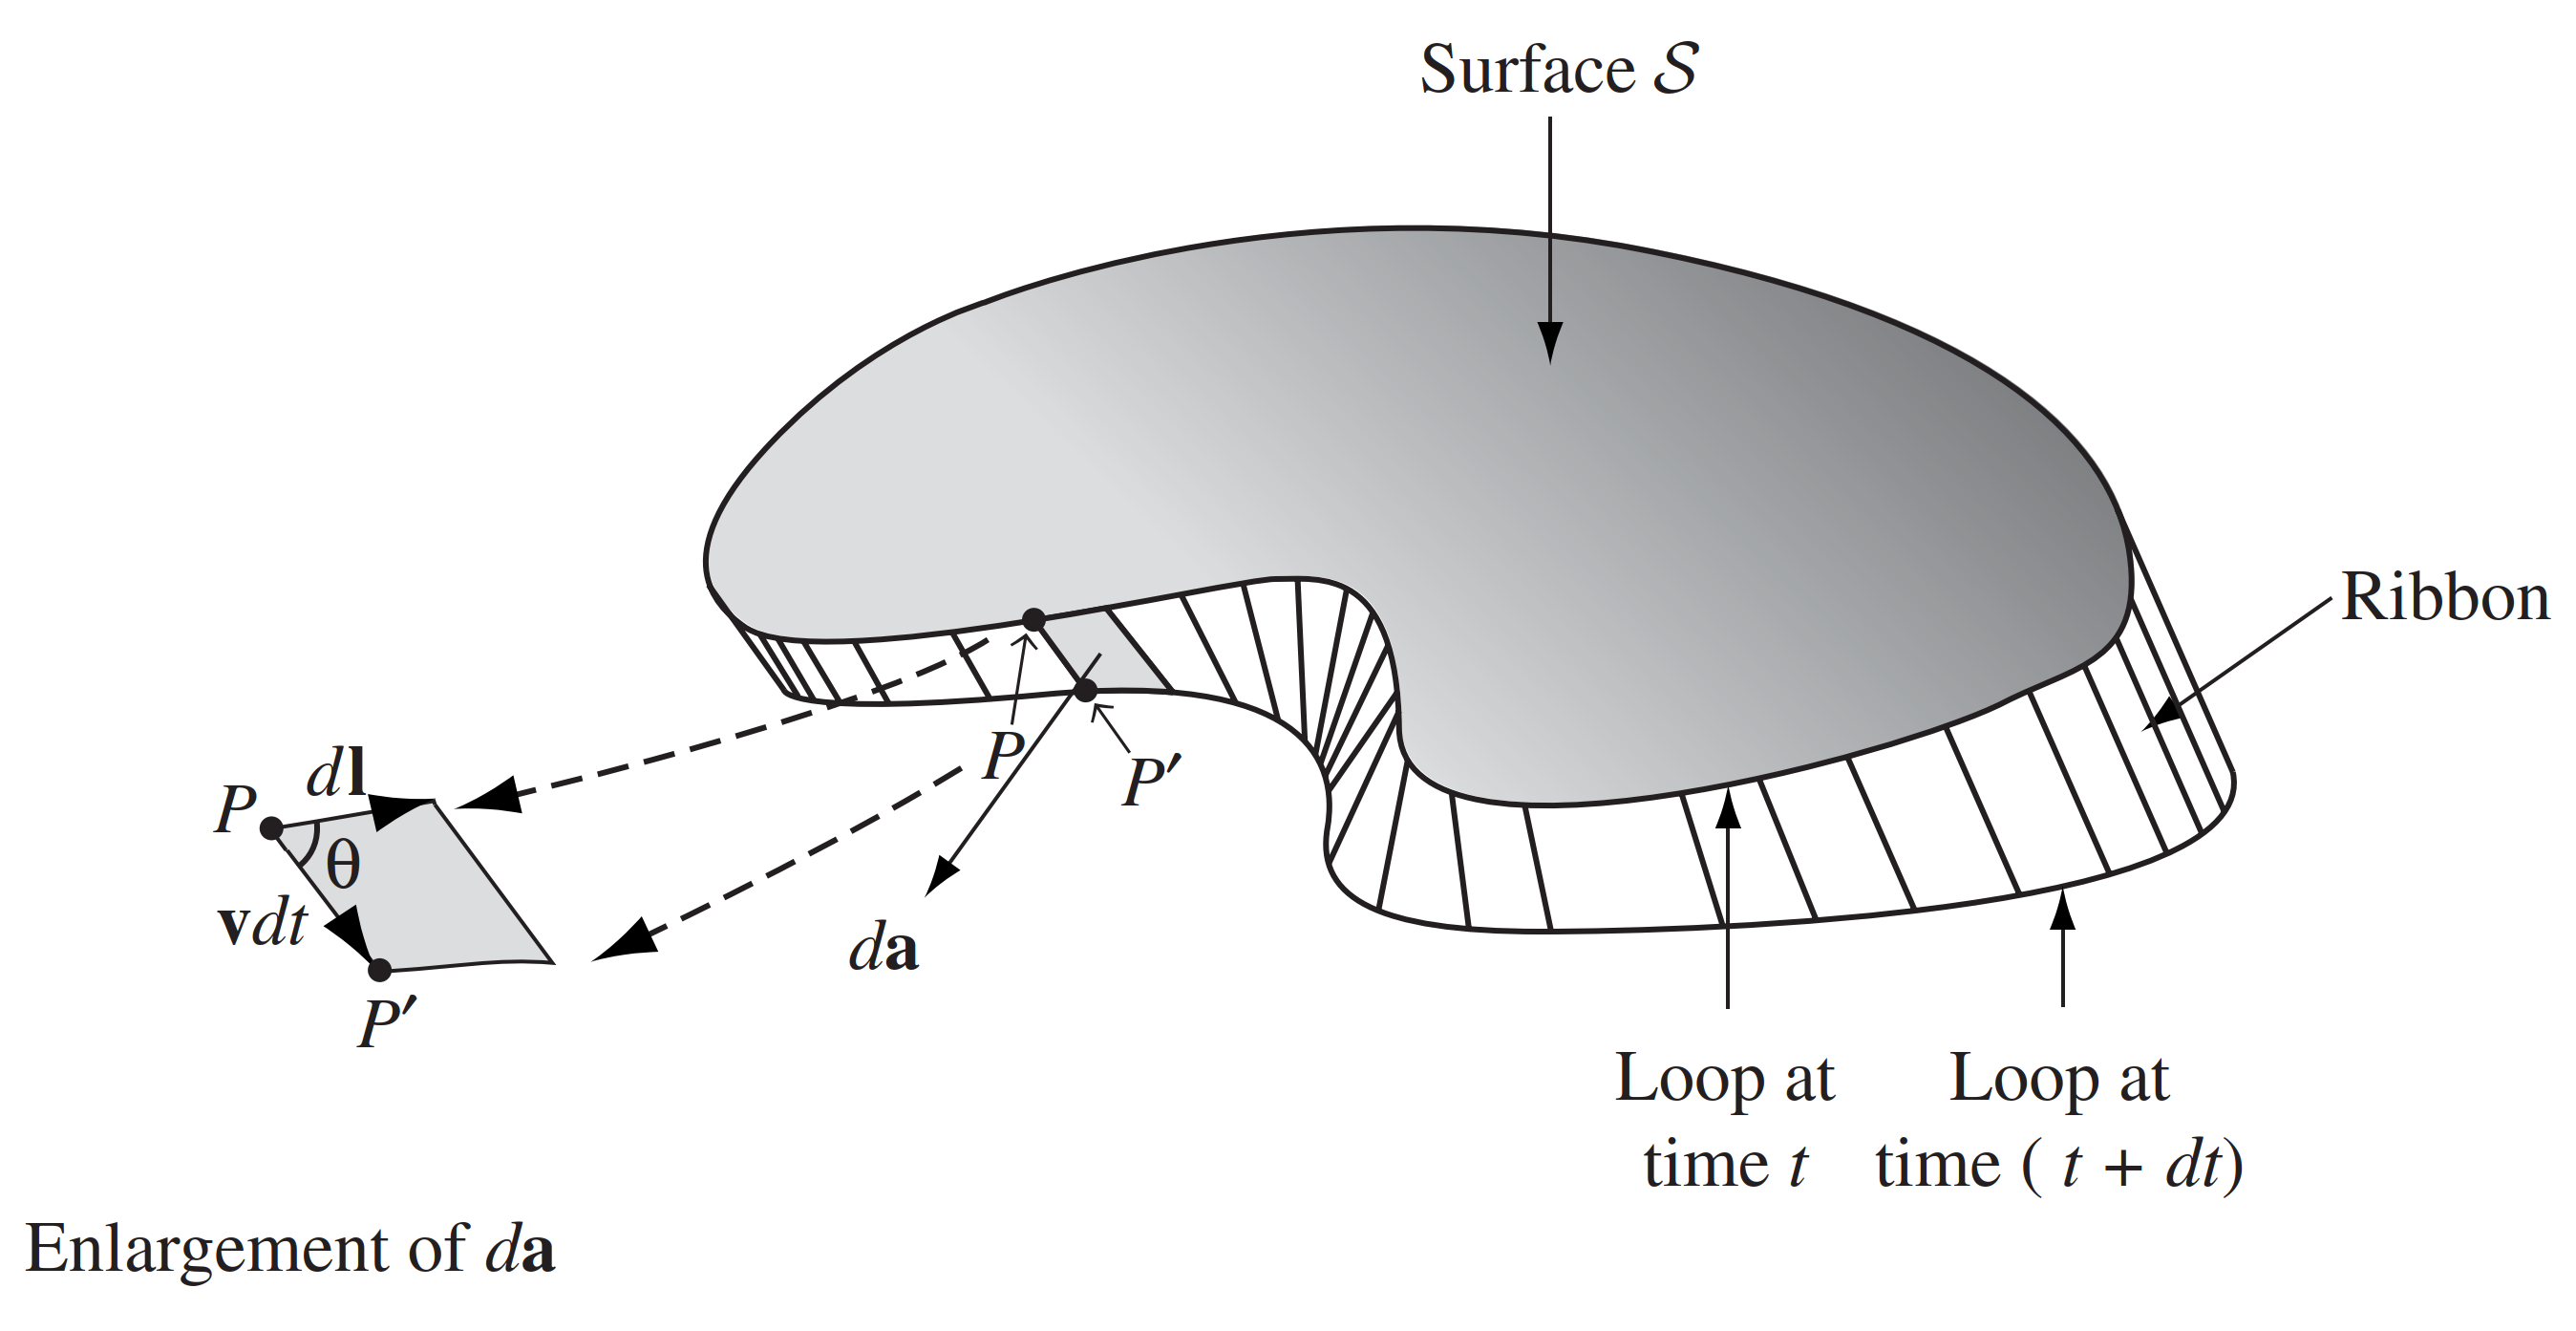
\includegraphics[width=0.85\textwidth]{../Rss/Electromagnetism/Electrodynamics/FluxRule.png}
    \caption*{Figure:  arbitrary loop of wire at time $t$, and also a short time $dt$ later}
\end{figure*}

\subsection*{Faraday's Law}
In 1831 Michael Faraday reported on a series of experiments, which resulted in an ingenious idea: A changing magnetic field induces an electric field. Indeed, if (as Faraday found empirically) the emf is again equal to the rate of change of the flux,
\begin{equation*}
    \upvarepsilon=\oint \mathbf{E}\cdot d\mathbf{l}=-\frac{d\Phi}{dt}
\end{equation*}
then \textbf{E} is related to the change in \textbf{B} by the equation
\begin{equation*}
    \oint \mathbf{E}\cdot d\mathbf{l}=-\int \frac{\partial \mathbf{B}}{\partial t}\cdot d\mathbf{a}
\end{equation*}
This is Faraday's law, in integral form. We can convert it to differential form by 
applying Stokes' theorem:
\begin{equation*}
    \nabla\times \mathbf{E}=-\frac{\partial \mathbf{B}}{\partial t}
\end{equation*}

For the first experiments, he pulled a loop of wire to the right through a magnetic field. A current flowed in the loop. This is, of course, is a straightforward case of motional emf $\upvarepsilon=-d\Phi/dt$. It’s  Lorentz force law at work; the emf is magnetic. For the second experiments, He moved the magnet to the left, holding the loop still. Again, a current flowed in the loop. This is what causes Faraday to think that changing magnetic field induces an electric field. The third, With both the loop and the magnet at rest, he changed the strength of the field (he used an electromagnet, and varied the current 
in the coil). Once again, current flowed in the loop. Because the magnetic field changes, it induces electric field, giving rise to an emf $-d\Phi/dt$. 

Viewed in this light, it is quite astonishing that all three processes yield the same formula for the emf. In fact, it was precisely this “coincidence” that led Einstein to the special theory of relativity—he sought a deeper understanding of what is, in classical electrodynamics, a peculiar accident. But that’s a story for another time.
\begin{figure*}[b]
    \centering
    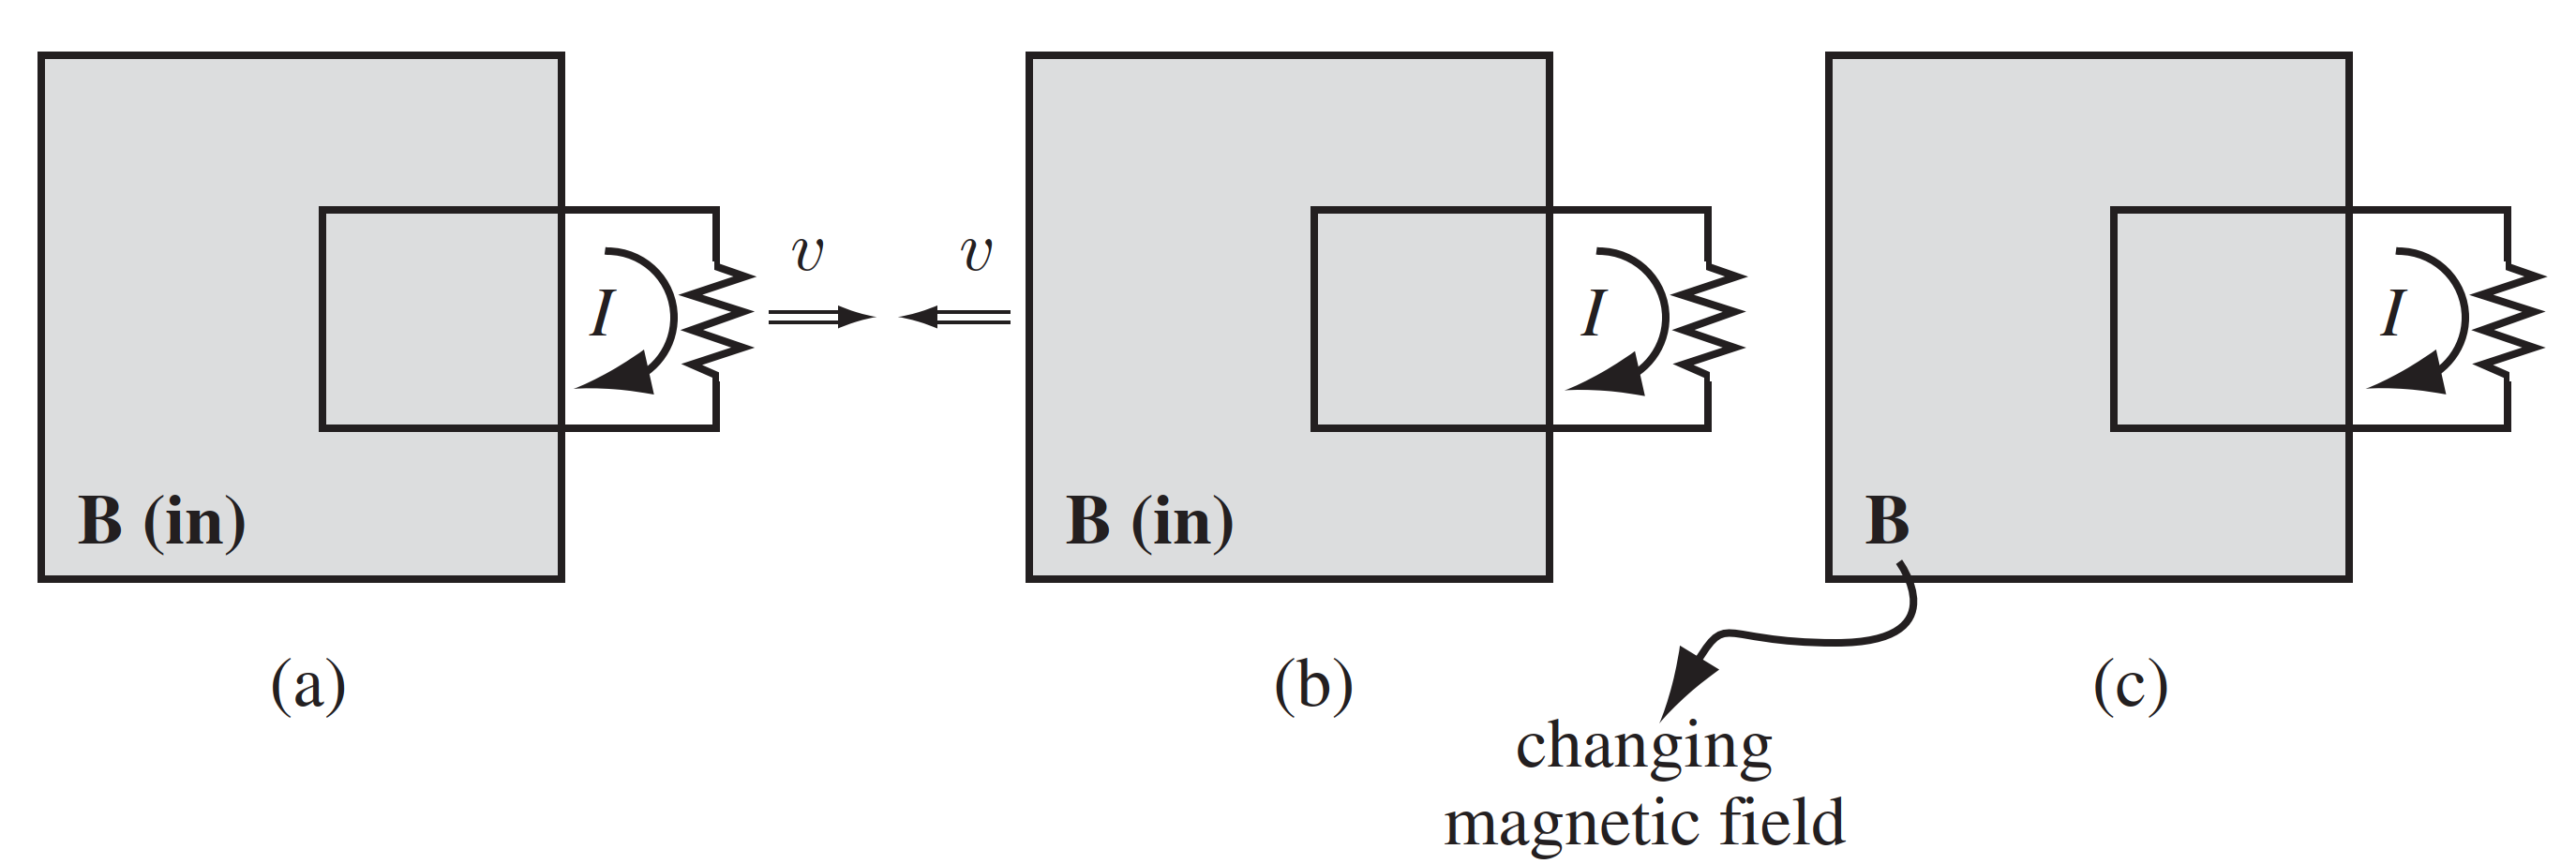
\includegraphics[width=0.85\textwidth]{../Rss/Electromagnetism/Electrodynamics/Faraday.png}
    \caption*{Figure: Faraday's experiments}
\end{figure*}

\subsubsection*{Lenz's Law.} Keeping track of the signs in Faraday’s law can be a real headache. But there’s a handy rule, called Lenz’s law, whose sole purpose is to help you get the directions right
\begin{equation*}
    \textbf{Nature abhors a change in flux.}
\end{equation*}
The induced current will flow in such a direction that the flux it produces tends to cancel the change. 

\subsection*{Inductance}
Suppose you have two loops of wire, at rest. If you run a steady current $I_1$ around loop 1, it produces a magnetic field $\mathbf{B}_1$. Some field lines pass through loop 2; let  $\Phi_2$ be the flux of $B_1$ through 2. You might have a tough time actually calculating $\mathbf{B}_1$, but a glance at the Biot-Savart law
\begin{equation*}
    \mathbf{B}_1=\frac{\mu_0I_1}{4\pi}\int \frac{d \mathbf{l}_1 \times\hrcurs}{\rcurs^2}
\end{equation*}
reveals one significant fact about this field: It is proportional to the current $I_1$. Therefore, so too is the flux through loop 2:
\begin{equation*}
    \Phi_2=\int \mathbf{B}_1\cdot d\mathbf{a}
\end{equation*}
Thus 
\begin{equation*}
    \Phi_2 = M_{21} I_1
\end{equation*}
where $M_21$ is the constant of proportionality; it is known as the mutual inductance of the two loops. Expressing the flux in terms of the vector potential, and invoking Stokes’ theorem
\begin{align*}
    \Phi_2 &=\int \nabla\times\mathbf{A}_1\cdot d\mathbf{a}_2\\
    &=\oint \mathbf{A}_1\cdot d\mathbf{l}_2\\
    &=\oint \frac{\mu_0I_1}{4\pi}\oint\frac{d\mathbf{l}_1}{\rcurs}\cdot d\mathbf{l}_2\\
    \Phi_2 &=\frac{\mu_0}{4\pi} \oint\oint\frac{d\mathbf{l}_1\cdot d\mathbf{l}_2}{\rcurs}I_1
\end{align*}
Evidently
\begin{equation*}
    M_{21}=\frac{\mu_0}{4\pi} \oint\oint\frac{d\mathbf{l}_1\cdot d\mathbf{l}_2}{\rcurs}
\end{equation*}
This is the Neumann formula; which is not very useful for practical calculations, but it does reveal two important things about mutual inductance:
\begin{enumerate}
    \item $M_21$ is a purely geometrical quantity, having to do with the sizes, shapes,
    and relative positions of the two loops.
    \item The integral  is unchanged if we switch the roles of loops 1 and 2; it follows that\begin{equation*}
        M_{21} = M_{12}
    \end{equation*} We may as well drop the subscripts and call them both M.
\end{enumerate} 
Suppose, now, that you vary the current in loop 1. The flux through loop 2 will vary accordingly, and Faraday’s law says this changing flux will induce an emf in loop 2:
\begin{equation*}
    \upvarepsilon=-\frac{\Phi_2}{dt}=-M\frac{dI_1}{dt}
\end{equation*}
Meaning, very time you change the current in loop 1, an induced current flows in loop 2--even though there are no wires connecting them! 

A changing current not only induces an emf in any nearby loops, it also induces an emf in the source loop itself. Once again, the field (and therefore also the flux) is proportional to the current:
\begin{equation*}
    \Phi=LI
\end{equation*}
The constant of proportionality $L$ is called the self inductance. If the current changes, the emf induced in the loop is
\begin{equation*}
    \upvarepsilon= -L\frac{dI}{dt}
\end{equation*}
Inductance is measured in henries (H); a Henry is a volt-second per ampere

\subsection*{Energy in Magnetic Fields}
The work done on a unit charge by you against the back emf, in one trip around the circuit is $-\upvarepsilon$. The amount of charge per unit time passing down the wire is $I $. So the total work done per unit time is
\begin{equation*}
    \frac{dW}{dt}=-\upvarepsilon I=LI\frac{dI}{dt}
\end{equation*}
If we start with zero current and build it up to a final value I, the work done
\begin{equation*}
    W=\frac{1}{2}LI^2
\end{equation*}
There is a nicer way to write $W$, which has the advantage that it is readily generalized to surface and volume currents
\begin{equation*}
    W=\frac{1}{2\mu_0}\bigg[\int_\mathcal{V} B^2\;d\tau-\oint \mathbf{A}\times \mathbf{B}\cdot d\mathbf{a}\bigg]
\end{equation*}
Now, the integration is to be taken over the entire volume occupied by the current, but \textbf{J} is zero out there anyway. In particular, if we agree to integrate over all space, then the surface integral goes to zero, and we are left with
\begin{equation*}
    W=\frac{1}{2\mu_0}\int B^2 \;d\tau\qquad\text{Over all Space}
\end{equation*}
In view of this result, we say the energy is “stored in the magnetic field,” in the amount
\begin{equation*}
    U_m=\frac{B^2}{\mu_0}
\end{equation*}
per unit volume. Although some might prefer to say that the energy is stored in the current distribution, in the amount $\frac{1}{2}\mathbf{A}\cdot\mathbf{J}$ per unit volume.

\subsection*{Maxwell's Equation}
Maxwell's equations, or Maxwell-Heaviside equations, are as follows
\begin{align*}
    \nabla\cdot\mathbf{E}&=\frac{1}{\epsilon_0}\rho\\
    \nabla\cdot\mathbf{B}&=0\\
    \nabla\times\mathbf{E}&=-\frac{\partial \mathbf{B}}{\partial t}\\
    \nabla\times\mathbf{B}&=\mu_0\mathbf{J}+\mu_0\epsilon_0\frac{\partial \mathbf{E}}{\partial t}
\end{align*}
or in integral form 
\begin{align*}
    \oint \mathbf{E}\cdot d\mathbf{a}&=\frac{1}{\epsilon}Q_\text{enc}\\
    \oint \mathbf{B}\cdot d\mathbf{a}&=0\\
    \oint \mathbf{E}\cdot d\mathbf{l}&=-\int \frac{\partial \mathbf{B}}{\partial t}\cdot d\mathbf{a}\\
    \oint \mathbf{B}\cdot d\mathbf{l}&=\mu_0\int\mathbf{J}\cdot d\mathbf{a}+ \mu_0\epsilon_0 \int\frac{\partial \mathbf{E}}{\partial t}\cdot d\mathbf{a}
\end{align*}

\subsubsection*{How Maxwell Fixed Ampère’s Law.} Ampère’s law is bound to fail for non-steady currents. Suppose we’re in the process of charging up a capacitor. In integral form, Ampère’s law reads
\begin{equation*}
    \oint \mathbf{B}\cdot d\mathbf{l}=\mu_0 I_\text{enc}
\end{equation*}
The total current passing through the loop, or, more precisely, the current piercing a surface that has the loop for its boundary. In this case, the simplest surface lies in the plane of the loop--the wire punctures this surface, so $I_\text{enc} = I$. Fine--but what if I draw instead the balloon-shaped surface? No current passes through this surface, and I conclude that $I_\text{enc} = 0$!

We will try to fix it by considering the continuity equation and  invoking Gauss's law
\begin{equation*}
    \nabla\cdot\mathbf{J}=-\frac{\partial \rho}{\partial t}=-\frac{\partial }{\partial t}(\epsilon_0 \nabla\cdot \mathbf{E})=-\nabla\cdot\epsilon_0\biggl(\frac{\partial \mathbf{E}}{\partial t}\biggr)
\end{equation*}
If we were to combine $\epsilon_0 \partial \mathbf{E}/\partial t$ with \textbf{J}, in Ampère’s law, it would be just right to kill off the extra divergence:
\begin{equation*}
    \oint \mathbf{B}\cdot d\mathbf{l} =\mu_0\int\mathbf{J}\cdot d\mathbf{a}+ \mu_0\epsilon_0 \int\frac{\partial \mathbf{E}}{\partial t}\cdot d\mathbf{a}
\end{equation*}

Apart from curing the defect in Ampère’s law, Maxwell’s term has a certain aesthetic appeal: Just as a changing magnetic field induces an electric field (Faraday’s law), a changing electric field induces a magnetic field.
\begin{figure*}[b]
    \centering
    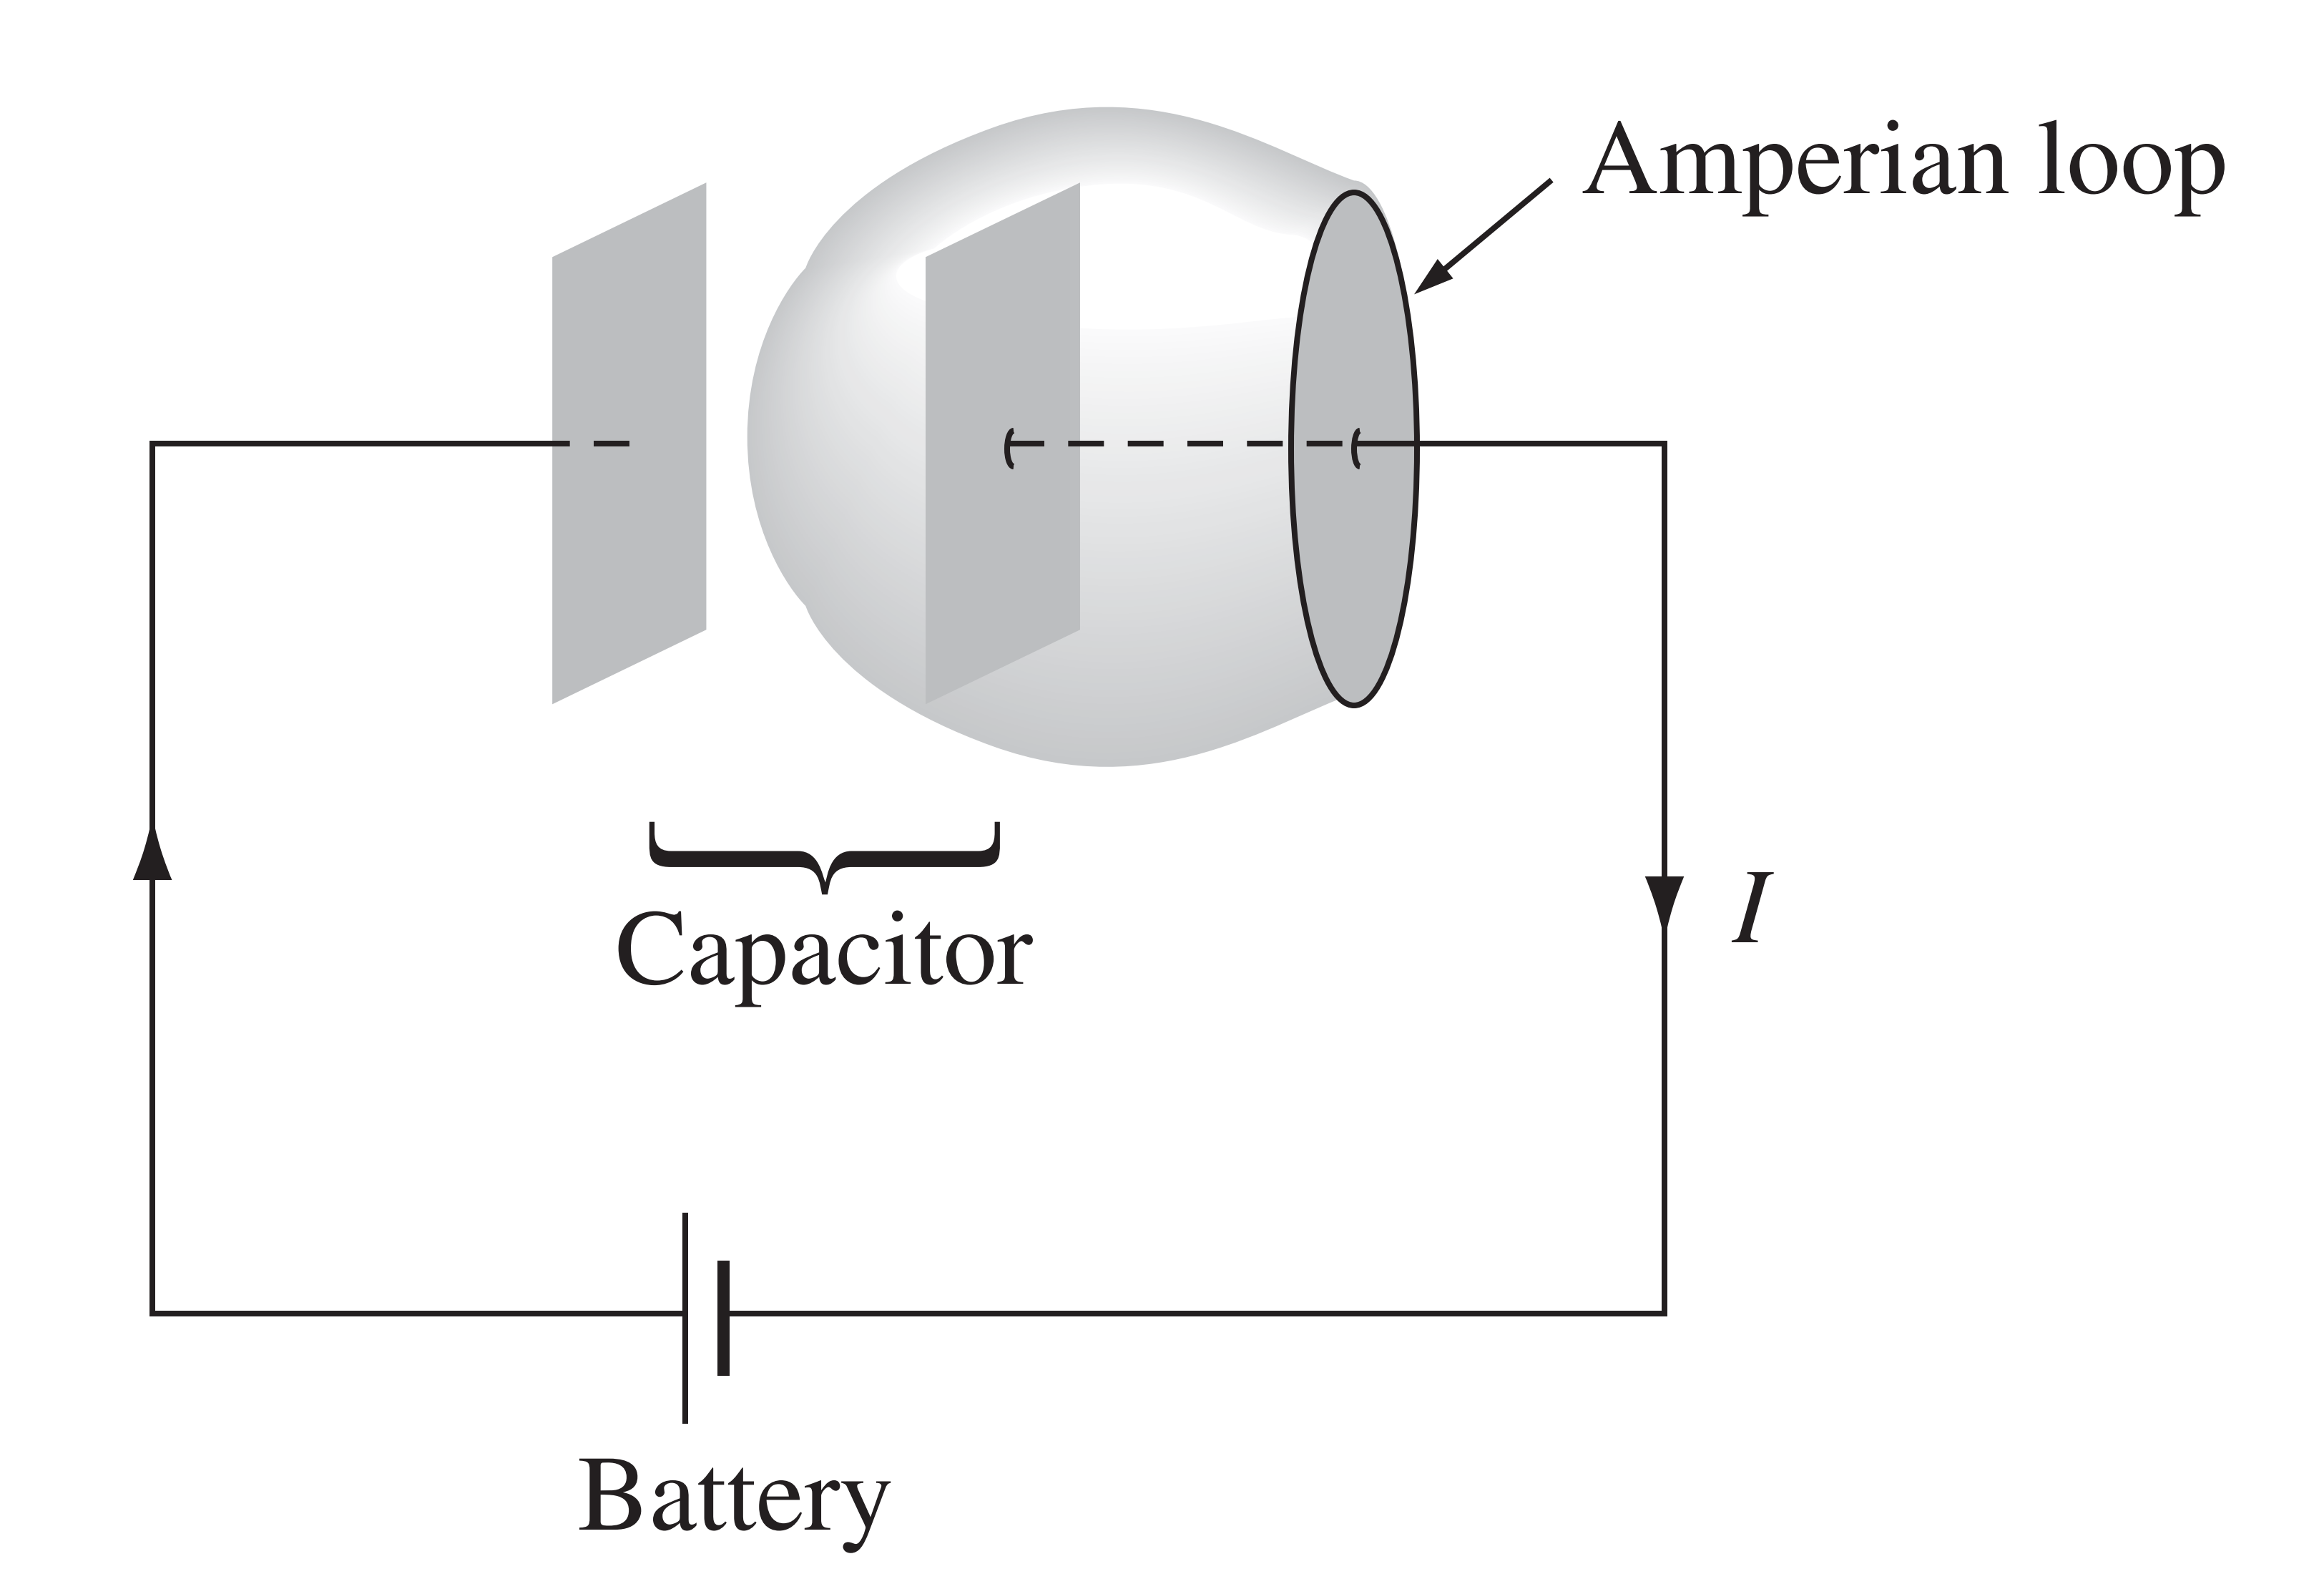
\includegraphics[width=0.65\textwidth]{../Rss/Electromagnetism/Electrodynamics/BrokenAmpereLaw.png}
\end{figure*}
\end{document}